\scanpage{51}

\uline{Lemma}\quad Let $A$ be a ring of endomorphisms of the abelian group $H^*(X)$, stable under homogeneous components (\uuline{total} degree), under transposition. \deleted{and} \inserted{Suppose $\xi\in A$, and} that for every $0\leq i<n$, there exists $u_i\in A$, \figure{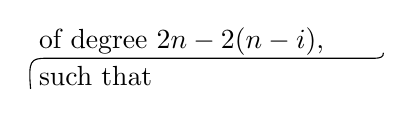
\begin{tikzpicture}[baseline=(t.base)]
\node[anchor=west,inner sep=0pt] (t) at (0,0) {such that};
\node[anchor=south west,inner sep=0pt] at (0,0.25) {\inserted{of degree $\deleted{2n}-2(n-i)$,}};
\draw (-0.10,-0.17) .. controls (-0.13,0.19) and (-0.10,0.22) .. (0.10,0.22) -- (4.25,0.22) .. controls (4.36,0.22) and (4.38,0.24) .. (4.38,0.29);
\end{tikzpicture}}
\[
u_i\xi^{n-i}:H^i(X)\longrightarrow H^{2n-i}(X)\longrightarrow H^{i}(X)
\]
is the identity.
\margin{\figure{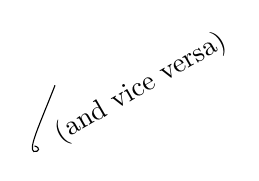
\begin{tikzpicture}[baseline=(v.base)]
\node[anchor=west,inner sep=0pt,rotate=30] (v) at (0,0) {(and vice versa)};
\draw (-0.02,0.65) .. controls (-0.22,0.14) and (-0.36,-0.15) .. (-0.29,-0.19) .. controls (-0.22,-0.20) and (-0.20,-0.14) .. (-0.28,-0.12);
\end{tikzpicture}}}
Then $A$ contains $L$!, \deleted{the $\pi$} and the projections onto the elementary factors $\xi^jP^i$ ($i\leq n$, and \deleted{and $i+2j\leq n$ \unsure{or} $i+2j\leq 2n-i$ \unsure{or}} $j\leq n-i$)

\uline{Corollary}\quad Equivalent conditions :

(i) $L$ Algebraic

(ii) for every $1\leq i\unsure{<|\leq}n$, there exists an \uline{algebraic} correspondence inducing $H^{2n-i}(X)\mathbin{-}H^i(X)$ inverse to $J^i$.

\deleted{(iii)} If this is so, then the \deleted{$\unsure{\xi}$} projections onto the elementary factors of $H^*(X)$, are algebraic, and the projections $H^*(X)\mathbin{-}H^i(X)$, too.

\uline{Proof of the lemma.}\quad Since $A$ stable under transposition, it suffices to look at the $\xi^jP^i$, for $i+2j\leq n$. Let $k=i+2j$. -- proceed by induction on $k$, trivial if $k<0$.

\mspage{50}
